% Created 2017-05-14 Sun 09:02
% Intended LaTeX compiler: pdflatex
\documentclass[presentation,10pt]{beamer}
\usepackage[utf8]{inputenc}
\usepackage[T1]{fontenc}
\usepackage{graphicx}
\usepackage{grffile}
\usepackage{longtable}
\usepackage{wrapfig}
\usepackage{rotating}
\usepackage[normalem]{ulem}
\usepackage{amsmath}
\usepackage{textcomp}
\usepackage{amssymb}
\usepackage{capt-of}
\usepackage{hyperref}
\usepackage{amsthm}
\usepackage{amsmath}
\usepackage{mathtools}
\newtheorem{mydef}{Definition}
\newtheorem{mythm}{Theorem}
\newcommand{\dx}{\mathrm{d}}
\newcommand{\var}{\mathrm{var}}
\newcommand{\cov}{\mathrm{cov}}
\newcommand{\corr}{\mathrm{corr}}
\newcommand{\pr}{\mathrm{Pr}}
\newcommand{\rarrowd}[1]{\xrightarrow{\text{ \textit #1 }}}
\DeclareMathOperator*{\plim}{plim}
\newcommand{\plimn}{\plim_{n \rightarrow \infty}}
\usepackage{booktabs}
\usepackage{color}
\setlength{\parskip}{1em}
\usetheme{CambridgeUS}
\usecolortheme{beaver}
\author{Zheng Tian}
\date{}
\title{Lecture 10: Nonlinear Regression Functions}
\hypersetup{
 pdfauthor={Zheng Tian},
 pdftitle={Lecture 10: Nonlinear Regression Functions},
 pdfkeywords={},
 pdfsubject={},
 pdfcreator={Emacs 25.1.1 (Org mode 9.0.3)}, 
 pdflang={English}}
\begin{document}

\maketitle
\begin{frame}{Outline}
\setcounter{tocdepth}{1}
\tableofcontents
\end{frame}



\section{Introduction}
\label{sec:org2327955}

\begin{frame}[label={sec:org7822a8a}]{Overview}
\begin{block}{Linear population regression function}
\(E(Y_i \mid \mathbf{X}_i) = \beta_0 + \beta_1 X_{i1} + \cdots + \beta_k
X_{ik}\), where \(\mathbf{X}_i = (X_{i1}, \ldots, X_{ik})^{\prime}\). 
\end{block}

\begin{block}{Nonlinear population regression function}
\(E(Y_i \mid \mathbf{X}_i) = f(X_{i1}, X_{i2}, \ldots, X_{ik};
\beta_1, \beta_2, \ldots, \beta_m)\), where \(f(\cdot)\) is a nonlinear function.
\end{block}

\begin{block}{Study questions}
\begin{itemize}
\item Why do we need to use nonlinear regression models?
\item What types of nonlinear regression models can we estimate by OLS?
\item How can we interpret the coefficients in nonlinear regression models?
\end{itemize}
\end{block}
\end{frame}

\section{A General Strategy For Modeling Nonlinear Regression Functions}
\label{sec:org0ea9900}

\begin{frame}[label={sec:org68f4a33}]{Test Scores and district income}
\begin{columns}
\begin{column}{0.4\columnwidth}
\begin{itemize}
\item Test scores can be determined by average district income

\item We estimate a simple linear regression model
\[TestScore = \beta_0 + \beta_1 Income + u\]

\item What's the problem with the simple linear regression model?
\end{itemize}
\end{column}
\begin{column}{0.6\columnwidth}
\begin{figure}[htbp]
\centering
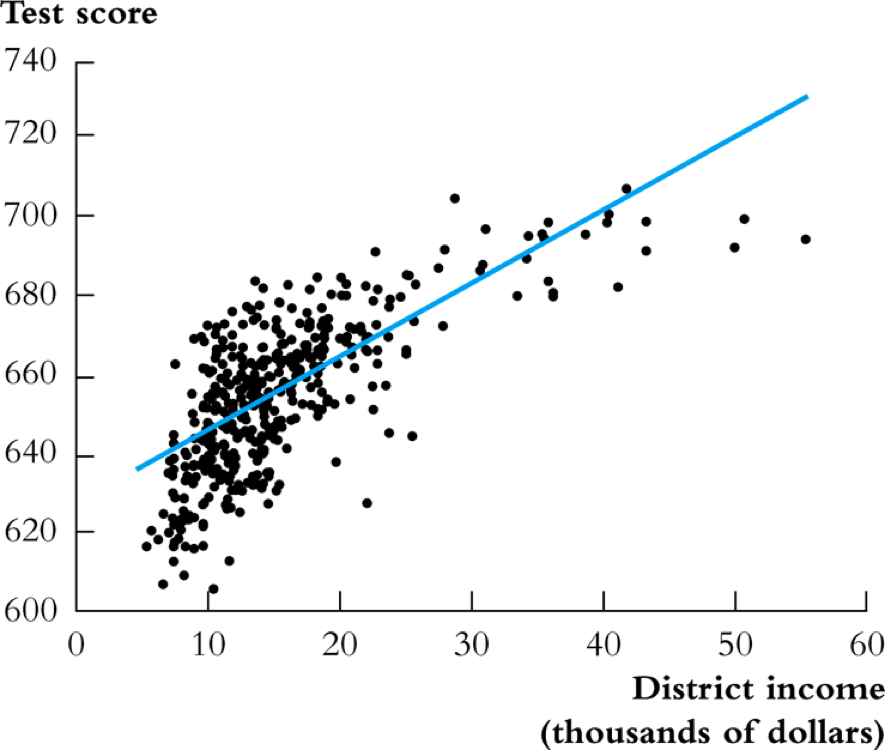
\includegraphics[width=0.85\textwidth]{img/fig-8-2.png}
\caption{\label{fig:orgb270522}
Scatterplot of test score vs district income and a linear regression line}
\end{figure}
\end{column}
\end{columns}
\end{frame}

\begin{frame}[label={sec:org47cc62f}]{Why does a simple linear regression model not fit the data well?}
\begin{itemize}
\item Data points are below the OLS line when income is very low (under
\$10,000) or very high (over \$40,000), and are above the line when
income is between \$15,000 and \$30,000.

\vspace{0.1cm}
\item The scatterplot may imply a curvature in the relationship between
test scores and income. 

\vspace{0.1cm}
That is, a unit increase in income may have larger effect on test
scores when income is very low than when income is very high.

\vspace{0.1cm}
\item The linear regression line cannot capture the curvature because the
effect of district income on test scores is constant over all the
range of income since 
\[\Delta TestScore / \Delta Income = \beta_1\]
where \(\beta_1\) is constant.
\end{itemize}
\end{frame}

\begin{frame}[label={sec:org6bcd308}]{Estimate a quadratic regression model}
\begin{equation}
\label{eq:quadratic-testscore}
TestScore = \beta_0 + \beta_1 Income + \beta_2 Income^2 + u
\end{equation}

\begin{itemize}
\item This model is nonlinear, specifically quadratic, with respect to
\(Income\) since we include the squared income.

\item The population regression function is
\[E(TestScore | Income) = \beta_0 + \beta_1 Income + \beta_2 Income^2\]

\item It is linear with respect to \(\beta\). So we can still use the
OLS estimation and carry out hypothesis testing as we do with a
linear regression model.
\end{itemize}
\end{frame}

\begin{frame}[label={sec:org8ef69b4}]{Estimate a quadratic regression model (cont'd)}
\begin{figure}[htbp]
\centering
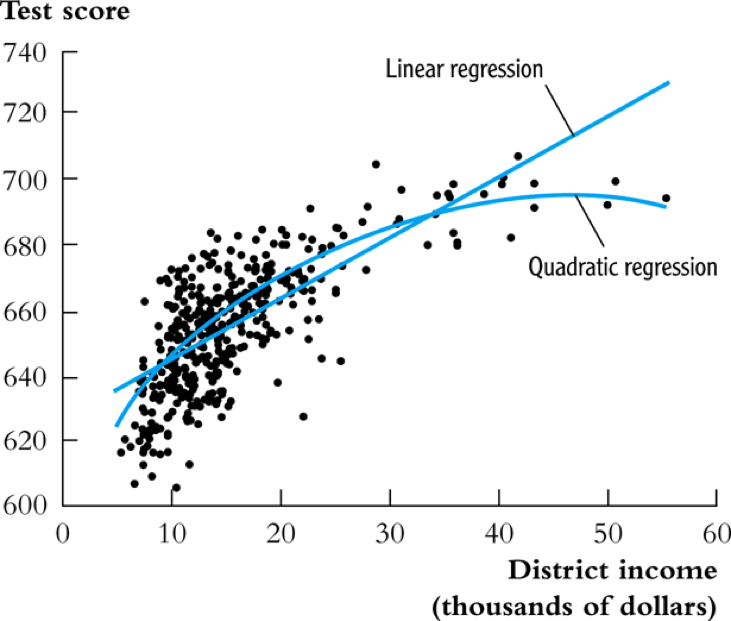
\includegraphics[width=0.6\textwidth,height=0.5\textwidth]{img/fig-8-3.png}
\caption{\label{fig:orge071eca}
Scatterplot of test score vs district income and a quadratic regression line}
\end{figure}
\end{frame}

\begin{frame}[shrink,label={sec:orge4e7589}]{A general formula for a nonlinear population regression function}
A general nonlinear regression model is

\begin{equation}
\label{eq:nl-general}
Y_i = f(X_{i1}, X_{i2}, \ldots, X_{ik}; \beta_1, \beta_2, \ldots, \beta_m) + u_i
\end{equation}

\begin{itemize}
\item The \alert{population nonlinear regression function}: 
\[ E(Y_i | X_{i1}, \ldots, X_{ik}) = f(X_{i1}, X_{2i}, \ldots, X_{ik}; \beta_1, \beta_2, \ldots, \beta_m) \]
\item The number of regressors and the number of parameters are not
necessarily equal in the nonlinear regression model.
\item In vector notation 
\begin{equation}
\label{eq:nl-general-mat}
Y_i = f(\mathbf{X}_i; \boldsymbol{\beta}) + u_i
\end{equation}
\item We focus on the nonlinear regression models
such that \(f(\cdot)\) is \alert{nonlinear with \(\mathbf{X}_i\)} but \alert{linear with
\(\boldsymbol{\beta}\)}.
\end{itemize}
\end{frame}

\begin{frame}[label={sec:org7d44912}]{The effect on \(Y\) of a change in a regressor}
For the general nonlinear model in Equation (\ref{eq:nl-general}), the
effect on \(Y\) of a change in one regressor, say \(X_1\), holding other
things constant, can be computed
as

\begin{equation}
\label{eq:nl-gen-effect}
\Delta Y = f(X_1 + \Delta X_1, X_2, \ldots, X_k; \boldsymbol{\beta}) - f(X_1, X_2, \ldots, X_k; \boldsymbol{\beta})
\end{equation}

When \(X_1\) and \(Y\) are continuous variables and \(f(\cdot)\) is
differentiable, the marginal effect of \(X_1\) is the partial derivative
of \(f\) with respect to \(X_1\), that is, holding other things constant

\[ \Delta Y = \frac{\partial f(X_1, \ldots, X_k; \boldsymbol{\beta})}{\partial X_1} \Delta X_1  \]
\end{frame}


\begin{frame}[label={sec:org1f5ddee}]{Application to test scores and income $\backslash$\ \small Estimation and inference}
We estimate the quadratic regression model for test scores and
district income (Equation \ref{eq:quadratic-testscore}) by OLS,
resulting in the following

\begin{equation}
\label{eq:tsr-income2}
\widehat{TestScore} = \underset{\displaystyle (2.9)}{607.3} +
\underset{\displaystyle (0.27)}{3.85}Income - \underset{\displaystyle (0.0048)}{0.0423}Income^2,\, \bar{R}^2 = 0.554
\end{equation}


We can test whether the squared income has a significant
coefficient. That is, we test \(H_0:\, \beta_2 = 0 \text{ vs. } H_1:\,
\beta_2 \neq 0\). In other words, we test the quadratic regression mode
against the linear regression model. For this two-sided test, we can
as usual compute the t-statistic

\[ t = \frac{-0.0423}{0.0048} = -8.81 > -1.96 \]

Thus, we can reject the null at the 1\%, 5\% and 10\% significance levels.
\end{frame}

\begin{frame}[shrink,label={sec:org00253e2}]{Application to test scores and income $\backslash$\ \small The effect of change in income on test scores}
\begin{block}{A change in income from \$10 thousand to \$20 thousand}
\begin{equation*}
\begin{split}
\Delta \hat{Y} &= \hat{\beta}_0 + \hat{\beta}_1 \times 11 + \hat{\beta}_2 \times 11^2 - (\hat{\beta}_0 + \hat{\beta}_1 \times 10 + \hat{\beta}_2 \times 10^2) \\
&= \hat{\beta}_1 (11 - 10) + \hat{\beta}_2(11^2 - 10^2) \\
& = 3.85 - 0.0423 \times 21 = 2.96
\end{split}
\end{equation*}
\begin{itemize}
\item Thus, the predicted difference in test scores between a district with
average income of \$11,000 and one with average income of \$10,000 is
2.96 points.
\end{itemize}
\end{block}

\begin{block}{A change in income from \$40 thousand to \$41 thousand}
\begin{equation*}
\begin{split}
\Delta \hat{Y} &= \hat{\beta}_0 + \hat{\beta}_1 \times 41 + \hat{\beta}_2 \times 41^2 - (\hat{\beta}_0 + \hat{\beta}_1 \times 40 + \hat{\beta}_2 \times 40^2) \\
&= \hat{\beta}_1 (41 - 40) + \hat{\beta}_2(41^2 - 40^2) \\
& = 3.85 - 0.0423 \times 81 = 0.42
\end{split}
\end{equation*}
\begin{itemize}
\item The predicted difference in test scores between a district with
average income of \$41,000 and one with average income of \$40,000 is
0.42 points.
\item A change of income of \$1,000 is associated with a
larger change in predicted test scores if the initial income is
\$10,000 than if it is \$40,000.
\end{itemize}
\end{block}
\end{frame}

\begin{frame}[label={sec:orgcd43514}]{A general approach to modeling nonlinearities using multiple regression}
\begin{enumerate}
\item Identify a possible nonlinear relationship.
\begin{itemize}
\item Economic theory
\item Scatterplots
\item Your judgment and experts' opinions
\end{itemize}
\item Specify a nonlinear function and estimate its parameters by OLS.
\begin{itemize}
\item The OLS estimation and inference techniques can be used as usual
when the regression function is linear with respect to \(\beta\).
\end{itemize}
\item Determine whether the nonlinear model improves upon a linear model
\begin{itemize}
\item Use t- and/or F-statistics to test the null hypothesis that the
population regression function is linear against the alternative
that it is nonlinear.
\end{itemize}
\item Plot the estimated nonlinear regression function.
\item Compute the effect on \emph{Y} of a change in \emph{X}.
\end{enumerate}
\end{frame}
\end{document}